\documentclass[a4paper,12pt]{article}\usepackage[]{graphicx}\usepackage[]{color}
%% maxwidth is the original width if it is less than linewidth
%% otherwise use linewidth (to make sure the graphics do not exceed the margin)
\makeatletter
\def\maxwidth{ %
  \ifdim\Gin@nat@width>\linewidth
    \linewidth
  \else
    \Gin@nat@width
  \fi
}
\makeatother

\definecolor{fgcolor}{rgb}{0.345, 0.345, 0.345}
\newcommand{\hlnum}[1]{\textcolor[rgb]{0.686,0.059,0.569}{#1}}%
\newcommand{\hlstr}[1]{\textcolor[rgb]{0.192,0.494,0.8}{#1}}%
\newcommand{\hlcom}[1]{\textcolor[rgb]{0.678,0.584,0.686}{\textit{#1}}}%
\newcommand{\hlopt}[1]{\textcolor[rgb]{0,0,0}{#1}}%
\newcommand{\hlstd}[1]{\textcolor[rgb]{0.345,0.345,0.345}{#1}}%
\newcommand{\hlkwa}[1]{\textcolor[rgb]{0.161,0.373,0.58}{\textbf{#1}}}%
\newcommand{\hlkwb}[1]{\textcolor[rgb]{0.69,0.353,0.396}{#1}}%
\newcommand{\hlkwc}[1]{\textcolor[rgb]{0.333,0.667,0.333}{#1}}%
\newcommand{\hlkwd}[1]{\textcolor[rgb]{0.737,0.353,0.396}{\textbf{#1}}}%
\let\hlipl\hlkwb

\usepackage{framed}
\makeatletter
\newenvironment{kframe}{%
 \def\at@end@of@kframe{}%
 \ifinner\ifhmode%
  \def\at@end@of@kframe{\end{minipage}}%
  \begin{minipage}{\columnwidth}%
 \fi\fi%
 \def\FrameCommand##1{\hskip\@totalleftmargin \hskip-\fboxsep
 \colorbox{shadecolor}{##1}\hskip-\fboxsep
     % There is no \\@totalrightmargin, so:
     \hskip-\linewidth \hskip-\@totalleftmargin \hskip\columnwidth}%
 \MakeFramed {\advance\hsize-\width
   \@totalleftmargin\z@ \linewidth\hsize
   \@setminipage}}%
 {\par\unskip\endMakeFramed%
 \at@end@of@kframe}
\makeatother

\definecolor{shadecolor}{rgb}{.97, .97, .97}
\definecolor{messagecolor}{rgb}{0, 0, 0}
\definecolor{warningcolor}{rgb}{1, 0, 1}
\definecolor{errorcolor}{rgb}{1, 0, 0}
\newenvironment{knitrout}{}{} % an empty environment to be redefined in TeX

\usepackage{alltt}
\usepackage{mathtools,amsfonts,amssymb,bm,cmbright, commath,multicol,fancyhdr, sansmath}
\usepackage[sfdefault,light]{roboto}
\DeclareMathOperator*{\argmin}{argmin}
\DeclareMathOperator*{\argmax}{argmax}

\pagestyle{fancy}
\fancyhf{}
\rhead{15/11/2016 ::: Nandan Rao}
\lhead{14D001 ::: Homework Set 2}
\rfoot{\thepage}
\IfFileExists{upquote.sty}{\usepackage{upquote}}{}
\begin{document}

\section*{Slides 6}

\subsection*{Problem 2.1}

The bernouli likelihood function, defined for random variable $t \in {-1,1}$, takes the form:
%
\begin{align*}
p(t = 1) &= p \\
p(t = -1) &= 1 - p
\end{align*}
%
If we now consider a sigmoid function $\sigma(u)$ which gives us a bernouli probability, $p \in [0,1]$, we then get the following:
%
\begin{align*}
p(t = 1) &= \sigma(u) \\
p(t = -1) &= 1 - \sigma(u)
\end{align*}
%
If we consider the situation where $\sigma(u)$ is the logistic function:
%
\begin{align*}
p(t = 1) &= \frac{1}{1 + e^{-u}} \\
p(t = -1) &= 1 - \frac{1}{1 + e^{-u}} \\
\end{align*}
%
The sigmoid/logistic function has the special property that in addition to have an output bounded between $[0,1]$, it's first derivative is also symmetric around 0. This is to say that from $[0, \infty]$, the function moves towards 1 at the exact same rate it moves towards 0 over the range $[0, -\infty]$. This implies the following:
%
$$
\sigma(u) = 1 - \sigma(-u)
$$
%
Using this, we can rewrite our previous pair of equations:
%
\begin{align*}
p(t = 1) &= \frac{1}{1 + e^{-u}} \\
p(t = -1) &= \frac{1}{1 + e^{u}} \\
\end{align*}
%
Or better still:
$$
p(t) = \frac{1}{1 + e^{-tu}}
$$
If we then plug the linear model $\bm{w}^T\phi(x) + b$ in for u, we find exactly the large margin classifier with the logistic loss function:
%
$$
p(t) = \frac{1}{1 + \exp \Big\{ -t(\bm{w}^T\phi(x) + b) \Big\} }
$$

\subsection*{Problem 2.2}

The MAP estimator is given, as per usual:
%
$$
w_{MAP} = \argmax_w p( \bm{t} | \bm{w}, X)p(\bm{w})
$$
%
Our $\bm{t}$ observed variables are bernouli $t \in {-1,1}$, and the linear model we are applying on our data to map it to our bernouli predictions is the logistic function. Our likelihood function $ p( \bm{t} | \bm{w}, X) $, is therefore exactly what we found in 2.1, while our prior on $\bm{w}$ is Gaussian. We include only the terms that are dependent on $\bm{w}$ and assume independence between rows of our design matrix:
%
\begin{align*}
w_{MAP} &= \argmax_w \prod_n \Bigg( \frac{1}{1 + \exp\Big\{ -t_n(\bm{w}^T{\phi}(x_n) + b)  \Big\} } \Bigg) * \exp \Big\{ -\frac{1}{2}\bm{w}^T \lambda N\ \bm{w} \Big\} \\
w_{MAP} &= \argmax_w \sum_n \Big( - \log \Big( 1 + \exp\Big\{  -t_n(\bm{w}^T{\phi}(x_n) + b)  \Big\} \Big)\Big) - \frac{\lambda N}{2}\bm{w}^T \bm{w} \\
w_{MAP} &= \argmin_w \sum_n \log \Big( 1 + \exp\Big\{ -t_n(\bm{w}^T{\phi}(x_n) + b)  \Big\} \Big) + \frac{\lambda }{2} \bm{w}^T \bm{w}
\end{align*}
%

Because $\log(1 + e^x)$ approximates $1 + e^x$, minimizing over these two is equivalent, and we have our solution.

\section*{Slides 7}

\subsection*{Problem 2}

The probability that a new point belongs to any given mixture k is the joint probability of that data and the latent variable that points to that particular mixture. We decompose this into the conditional probability of the data given that particular mixture multiplied by the prior on the probability of that mixture. To coerce this into a probability, we normalize by the sum of the probabilities that the point belongs to each mixture k:
%
\begin{align*}
\Pi_k &= \frac{p(x_{n+1}, z_k)}{\sum_i^K p(x_{n+1} | z_i)} \\
\Pi_k &= \frac{p(x_{n+1} | z_k)p(z_k)}{\sum_i^K p(x_{n+1} | z_i)}
\end{align*}
%
We will focus on determining the formula for the numerator, for one particular k, as this is simply repeated for all k's to create a vector of probabilities, and the denominator follows directly from the numerator. The latent variable $z_k$ corresponds to the mean $\mu_k$ and precision $Q_k$ for that particular guassian, so we compute the probability that $x_{n+1}$ came from that gaussian, multiplied by whatever our prior probability was on that gaussian (we could assume this is a):
%
$$
p(x_{n+1} | z_k)p(z_k)
$$
$$
\frac{exp \Big\{ -\frac{1}{2} (x_{n+1} - \mu_k)^T Q (x_{n+1} - \mu_k) \Big\} }{\sqrt{|2\pi Q^{-1}|}} * p(z_k)
$$
\subsection*{Problem 5}

\subsubsection*{Robust Regression}

Assuming $\nu$ is fixed and applying bayes theorum:
%
\begin{align*}
p( \eta_n | t_n, \nu ) &= \frac{p(t_n | \nu, \eta_n) p(\eta_n | \nu)}{p(t_n, \nu)}
\end{align*}
%
In robust regression we model the observed data, $\bm{t}$, as gaussian, but where the gaussian for every observation has a variance derived from a latent variable $\eta_n$ which itself is a random variable picked from a gamma distribution. Because the gamma is a conjugate prior for the precision of the gaussian distribution, we end with a gamme distribution of the form, which we shall provide later in its full, ugly, PDF form, and therefore spare the reader at this point. Suffice to say at this juncture that we increase the $\alpha$ parameter by a half, and the $\beta$ paramter by half the squared residuals:
\begin{align*}
p( \eta_n | t_n, \nu ) \thicksim \mathit{Gamma}((\nu + 1)/2, (\nu + q(t_n - \phi(\bm{x}_n)^T\bm{w})^T(t_n - \phi(\bm{x}_n)^T\bm{w})/2 - 1))
\end{align*}

\subsubsection*{Logistic and Probit Models}
%
We will consider a general case of K discrete possible values for $t$, which will easily hold true for our binomial case, and will be shown to be a more general expression of the truncated distribution in the currently-considered binomial case. We can marginalize over $t$:
%
$$
p(z_n | \bm{w}, \bm{x}_n) = \sum_k p(z_n | \bm{w}, \bm{x}_n, t_k)p(t_k | \bm{w}, \bm{x}_n)
$$
%
Expanding the sum over possible values of $t$, and gathering terms, we come to:
%
\begin{align*}
p(z_n | \bm{w}, \bm{x}_n, t_n) &= \frac{p(z_n | \bm{w}, \bm{x}_n) - \sum_{k \neq n}^K p(z_n | \bm{w}, \bm{x}_n, t_k)p(t_k | \bm{w}, \bm{x}_n)}{p(t_n | \bm{w}, \bm{x}_n)}
\end{align*}
%
We gather the marginal distributions into their joint distribution as follows:
%
\begin{align}
p(z_n | \bm{w}, \bm{x}_n, t_n) &= \frac{p(z_n | \bm{w}, \bm{x}_n) - \sum_{k \neq n}^K p(z_n, t_k | \bm{w}, \bm{x}_n)}{p(t_n | \bm{w}, \bm{x}_n)}
\end{align}
%
We can begin to see some things in the above equation that match our intuition, and similarly match the definition of a truncated distribution, where we have turned a continous distribution function into a piece-wise function that returns 0 over certain intervals. For any $z_n$ that deterministically gives us $t_k$:
%
$$
p(z_n | \bm{w}, \bm{x}_n) = p(z_n, t_k | \bm{w}, \bm{x}_n)
$$
%
Together with our (1), this gives us the desired result that for any $z_n$ that deterministically gives us $t_k$, where $t_k \neq t_n$:
%
$$
p(z_n | \bm{w}, \bm{x}_n, t_n) = 0
$$
np%
This gives us a probability function that will return 0 for any $z_n$ outside of the range of the $t_n$ it is conditioned upon, and for every other value of $z_n$ will return:
%
\begin{align}
p(z_n | \bm{w}, \bm{x}_n, t_n) &= \frac{p(z_n | \bm{w}, \bm{x}_n)}{\int p(t_n | \bm{w}, \bm{x}_n, z_n)p(z_n)dz}
\end{align}
%
It is easy to see that through the defined relationship, $t_n = 1[z_n > 0]$, $p(t_n | \bm{w}, \bm{x}_n, z_n)$ is deterministic, and therefore marginilizing over the $p(z_n)$ is equal to the probability given by the CDF of $p(z_n | \bm{w}, \bm{x}_n)$ of $z_n$ being within the range of $t_n$, which relates back to the truncated distribution over $z_n$, which attempts to scale up the probabilities within the range by the amount of total distributed mass outside the range. We therfore have another way to express this function, which is useful:
%
\begin{align*}
p(z_n | \bm{w}, \bm{x}_n, t_n = 0) &\thicksim \mathit{TruncatedNormal}(\phi(\bm{x}_n)^T\bm{w}, \sigma^2, (-\infty, 0])
\end{align*}
Now that we have seen the whole pictures, we can easily define the probability in our binary casein regards to a PDF g(x), based on scaling the probability of a given $z_n$ by the CDF of $z$ over the defined distribution for $t_n$:
\begin{align*}
p(z_n | \bm{w}, \bm{x}_n, t_n = 0) &= \frac{ g(z_n, \bm{x}_n, \bm{w})}{ \int_{-\infty}^{0} g(z_n, \bm{x}_n, \bm{w})  dz} \\
p(z_n | \bm{w}, \bm{x}_n, t_n = 1) &= \frac{ g(z_n, \bm{x}_n, \bm{w})}{ \int_{0}^{\infty} g(z_n, \bm{x}_n, \bm{w})  dz}
\end{align*}
We then defin g(x) for each distribution, for the probit, it is a gaussian PDF:
\begin{align*}
g(z_n, \bm{x}_n, \bm{w}) &= \frac{1}{\sqrt{2\pi\sigma^2}} \exp \Big\{  - \frac{(z_n - \phi(\bm{x}_n)\bm{w})^2}{2\sigma^2} \Big\}
\end{align*}
And for the logistic, we are given the PDF as follows:
\begin{align*}
g(z_n, \bm{x}_n, \bm{w}) &= \frac{e^{ \phi(\bm{x}_n)^T\bm{w}}}{(1 + e^{ \phi(\bm{x}_n)^T\bm{w}})^2}
\end{align*}
\subsubsection*{Gaussian Mixture Models}

The probability of
$$
z_n | \bm{x}_n, \bm{\mu}_{1:K}, \bm{Q}_{1:K}
$$
Is the latent variable for each observation, that contains the ``responsibility'' that each gaussian mixture, K, has over the variable. This is a vector that consists of the following for each K:
\begin{align*}
\Pi_k &= \frac{p(x_{n+1}, z_k)}{\sum_i^K p(x_{n+1} | z_i)}
\end{align*}


\subsubsection*{Factor Model}

Applying bayes theorum and assuming independence of parameters:
%
\begin{align*}
p( \bm{z}_n | \bm{x}_n, \bm{w}, \bm{\Sigma} ) &= \frac{p(\bm{x}_n | \bm{z}_n, \bm{w}, \bm{\Sigma}) p(\bm{z}_n, \bm{w}, \bm{\Sigma})} {p(\bm{x}_n, \bm{w}, \bm{\Sigma})} \\
p( \bm{z}_n | \bm{x}_n, \bm{w}, \bm{\Sigma} ) &= \frac{p(\bm{x}_n | \bm{z}_n, \bm{w}, \bm{\Sigma}) p(\bm{z}_n)} {p(\bm{x}_n | \bm{w}, \bm{\Sigma})}
\end{align*}
%
Focusing on the numerator (we can recover the normalizing constant later, as per usual), we see that we have the multiplication of two provided normal distributions, seeing as:
$$
\bm{x}_n | \bm{z}_n, \bm{w}, \bm{\Sigma} \thicksim \mathcal{N}(\bm{\mu} + \bm{W}\bm{z}_n\bm{\Sigma}) \ \ \ \  \bm{z}_n \thicksim \mathcal{N}(\bm{0}_R, \bm{I}_R)
$$
We know that the conditional distribution of two gaussians is also gaussian. Bishop provides us with a handy rule for finding the conditional distribution of two gaussians, which we will employ here:
\begin{align*}
P &= \bm{I}_R + \bm{W}^T\bm{\Sigma}^{-1}\bm{W} \\
G &= \bm{W}^T\bm{\Sigma}^{-1}(\bm{x}_n - \bm{\mu}) + \bm{I}_R^{-1}\bm{0}_R \\
&= \bm{W}^T\bm{\Sigma}^{-1}(\bm{x}_n - \bm{\mu})\\
p( \bm{z}_n &| \bm{x}_n, \bm{w}, \bm{\Sigma} ) \thicksim \mathcal{N}(P^{-1}G, P^{-1})
\end{align*}
%
\section*{Slides 8}

\subsection*{Problem 1}

We begin with bayes theorum, and rearrange taking advantage of indepence of parameters and expressing the marginal distribution denominator as the joint distribution of our observed variable with our latent variable, integrated over our latent variable:
%
\begin{align*}
p(\eta_n | \bm{t}_n, \bm{X}_n, \bm{w}, q) &= \frac{ p(\bm{t}_n | \eta_n, X_n, \bm{w}, q) p(\eta_n, \bm{X}_n, \bm{w}, q)  }{ p(\bm{t}_n, \bm{X}_n, \bm{w}, q )} \\
p(\eta_n | \bm{t}_n, \bm{X}_n, \bm{w}, q) &= \frac{ p(\bm{t}_n | \eta_n, X_n, \bm{w}, q) p(\eta_n)  }{ \int p(\bm{t}_n, | \eta_n, \bm{X}_n, \bm{w}, q )p(\eta_n) d\eta }
\end{align*}
%
We will focus first on simplifying our numerator, $p(\bm{t}_n | \eta_n, X_n, \bm{w}, q) p(\eta_n)$. We plug in the given distributions for $\bm{t}_n$ and $/eta_n$ and combine terms:
%
$$
\frac{ (\frac{\nu}{2} - 1)^{\frac{\nu}{2}} \eta^{\frac{\nu}{2} - 1} }{ \Gamma(\frac{\nu}{2}) }
\exp \Bigg\{  -\eta(\frac{\nu}{2} - 1)   \Bigg\}
\frac{1}{| 2\pi(\eta q)^{-1} \bm{I} |^{ \frac{1}{2}}}
\exp \Bigg\{  -\frac{\eta q}{2} (\phi(\bm{X}_n)^{T}\bm{w})^T(\phi(\bm{X}_n)^T\bm{w})   \Bigg\}
$$
$$
\frac{ (\frac{\nu}{2} - 1)^{\frac{\nu}{2}} \eta^{\frac{\nu}{2} - 1} }{ \Gamma(\frac{\nu}{2}) (2\pi)^{ \frac{1}{2}} \eta^{- \frac{1}{2}} q^{- \frac{1}{2} } }
\exp \Bigg\{ -\eta(\frac{\nu}{2} - 1 + \frac{q}{2} (\phi(\bm{X}_n)^{T}\bm{w})^T(\phi(\bm{X}_n)^T\bm{w}))   \Bigg\}
$$
$$
\frac{ q^{ \frac{1}{2}} (\frac{\nu}{2} - 1)^{\frac{\nu}{2}} \eta^{\frac{\nu + 1}{2} - 1} } { \Gamma(\frac{\nu}{2}) (2\pi)^{ \frac{1}{2}} }
\exp \Bigg\{ -\eta(\nu + q (\phi(\bm{X}_n)^{T}\bm{w})^T(\phi(\bm{X}_n)^T\bm{w})/2 - 1)   \Bigg\}
$$
%
At this point we see that we have found our $\beta$ in the exponent term, and in our $\eta$ term, which is great. We also see that we have a $sqrt{\pi}$, which we know is equal to $\Gamma(\frac{1}{2})$. Safe to say, that attempting to perform the integration at this point would be a waste of my youth. I will go ahead and skip to the following:
%
$$
C * \eta^{\frac{\nu + 1}{2} - 1} *
\exp \Bigg\{ -\eta(\nu + q (\phi(\bm{X}_n)^{T}\bm{w})^T(\phi(\bm{X}_n)^T\bm{w})/2 - 1)   \Bigg\}
$$
$$
 \thicksim \mathit{Gamma}((\nu + 1)/2, (\nu + q(t_n - \phi(\bm{x}_n)^T\bm{w})^T(t_n - \phi(\bm{x}_n)^T\bm{w})/2 - 1))
$$
\subsection*{Problem 2}

We start from the following definition:

\begin{align*}
\int \log p(\bm{t}, \bm{\eta | \theta}) p(\bm{\eta} | \bm{t}, \theta')d\bm{\eta} + C
\end{align*}

With C referring to everything that does not depend on $\theta$. Quite luckily, we have already derived the joint distribution of $t_n$ and $\eta$, and we can substitute everything there that does not depend on $\theta$, which is the exponent term, which of course cancels the log:


$$
\int -\eta(\nu + q (\phi(\bm{X}_n)^{T}\bm{w})^T(\phi(\bm{X}_n)^T\bm{w})/2 - 1) p(\bm{\eta} | \bm{t}, \theta')d\bm{\eta} + C
$$
$$
\int -(\nu + q (\phi(\bm{X}_n)^{T}\bm{w})^T(\phi(\bm{X}_n)^T\bm{w})/2 - 1) \bm{\eta} p(\bm{\eta} | \bm{t}, \theta')d\bm{\eta} + C
$$
$$
\int -(\nu + q (\phi(\bm{X}_n)^{T}\bm{w})^T(\phi(\bm{X}_n)^T\bm{w})/2 - 1) \mathbb{E}[\bm{\eta} | \bm{t}, \bm{X}, \theta'] + C
$$
%

\subsection*{Problem 3}

\subsubsection*{1}

Code is included in the appendix, here are the juicy plots that show how much more certain we are about our weights in the robust regresssion:


\begin{knitrout}
\definecolor{shadecolor}{rgb}{0.969, 0.969, 0.969}\color{fgcolor}
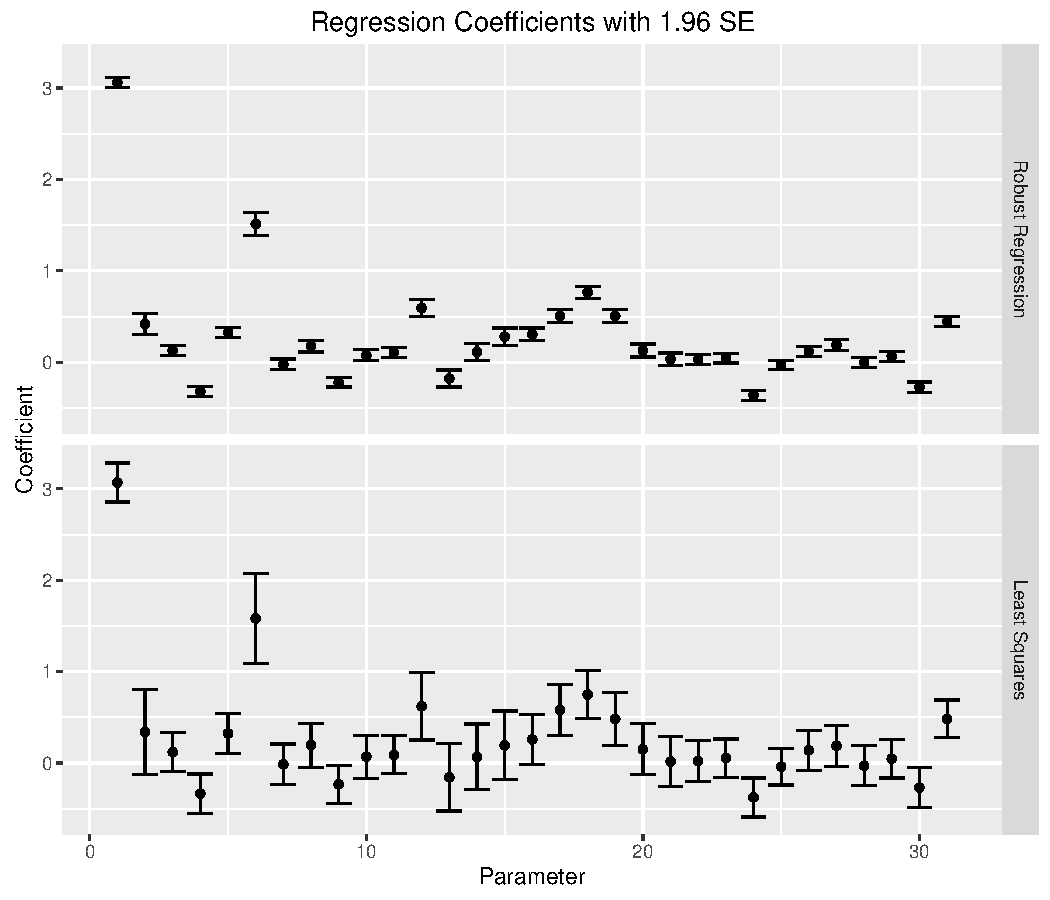
\includegraphics[width=\maxwidth]{figure/coefficients-1} 

\end{knitrout}


\subsubsection*{2}
%
Here we can see that the data does not at all fit with the OLS assumption of gaussian errors distributed by the sample variance!

\begin{knitrout}
\definecolor{shadecolor}{rgb}{0.969, 0.969, 0.969}\color{fgcolor}
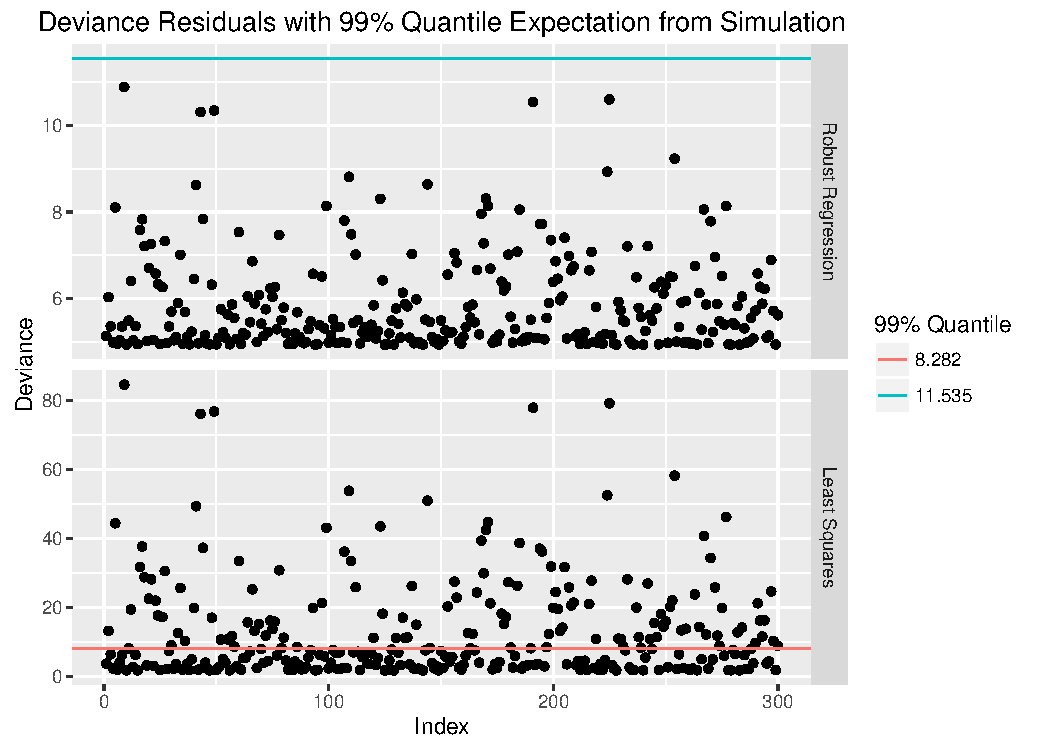
\includegraphics[width=\maxwidth]{figure/deviance-1} 

\end{knitrout}

\subsubsection*{3}

One simple idea is to track the loglikelihood of the parameters at every given iteration, and stop when the change between the current iteration and the last drops below a certain tolerance level. You can see this implemented in the code in the appendix, but here is a graph showing difference possible tolerance level cutoffs one could pick, in regards to the loglikelihood of the model:

\begin{knitrout}
\definecolor{shadecolor}{rgb}{0.969, 0.969, 0.969}\color{fgcolor}
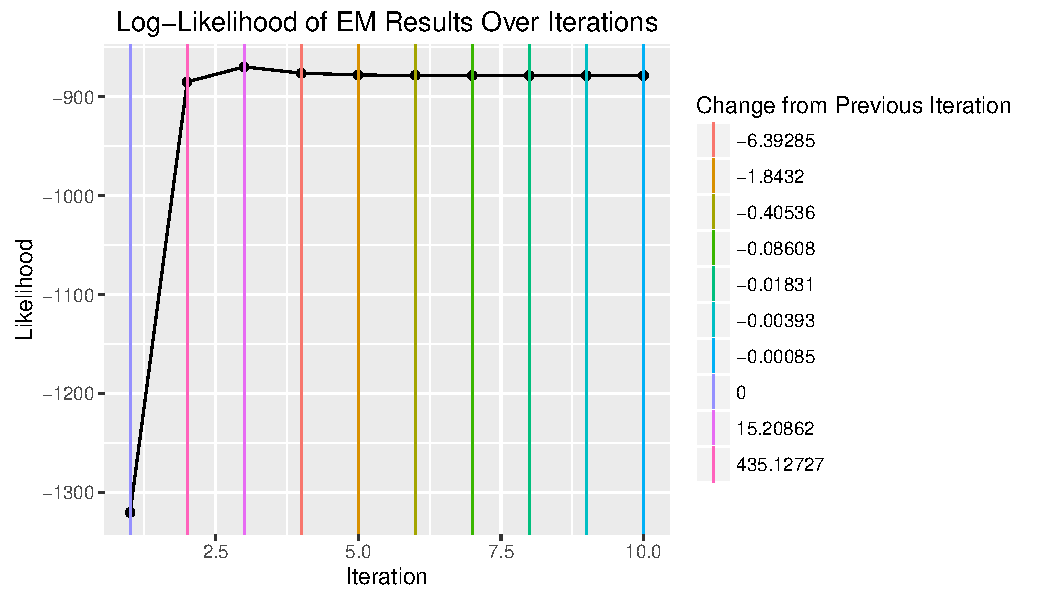
\includegraphics[width=\maxwidth]{figure/loglikelihood-1} 

\end{knitrout}


\subsubsection*{4}

Estimating the hyperparameter, $\nu$, can be done in a number of ways. One way could be to put a prior on the hyperparameter itself, a hyperprior, and try and learn the parameter from the data. This would not lead to the sample analytical solution for the above implementation, but one could trivially implement this using MCMC.  Another option is to use cross validation to try a number of different hyperparameters, and pick the one that gives the best results. This becomes a basic model-selection process. Plotted we have different $\nu$ values and their cross-validated SSE using k-fold cross validation with K = 5. This shows that a choice of 10 is actually very sensible!

\begin{knitrout}
\definecolor{shadecolor}{rgb}{0.969, 0.969, 0.969}\color{fgcolor}
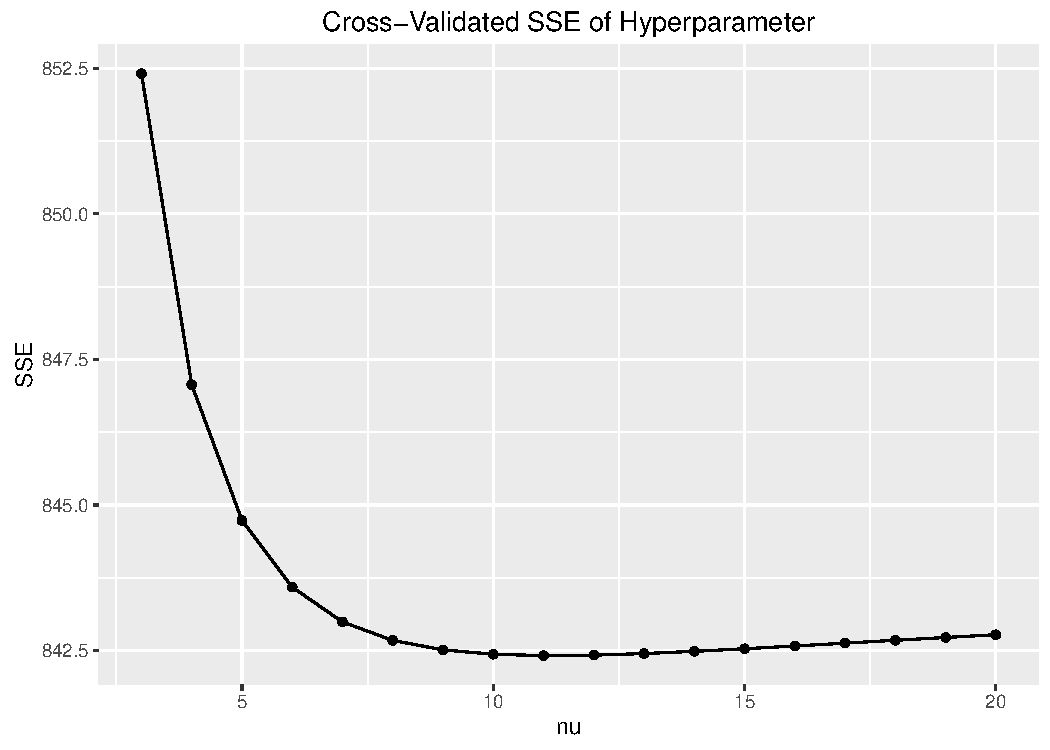
\includegraphics[width=\maxwidth]{figure/nu-1} 

\end{knitrout}

\appendix
\section{Source Code}

\begin{knitrout}\scriptsize
\definecolor{shadecolor}{rgb}{0.969, 0.969, 0.969}\color{fgcolor}\begin{kframe}
\begin{alltt}
\hlcom{################### LOAD ####################################}
\hlkwd{load}\hlstd{(}\hlstr{"synth_reg.rda"}\hlstd{)}
\hlkwd{library}\hlstd{(dplyr)}
\hlkwd{library}\hlstd{(ggplot2)}
\hlkwd{library}\hlstd{(MASS)}

\hlstd{em} \hlkwb{<-} \hlkwa{function} \hlstd{(}\hlkwc{T}\hlstd{,} \hlkwc{X}\hlstd{,} \hlkwc{iter} \hlstd{=} \hlnum{10}\hlstd{,} \hlkwc{nu} \hlstd{=} \hlnum{10}\hlstd{,} \hlkwc{tol}\hlstd{=}\hlnum{10}\hlopt{**-}\hlnum{3}\hlstd{) \{}

    \hlcom{# Initialize our theta variables}
    \hlstd{q} \hlkwb{<-} \hlnum{1}
    \hlstd{w} \hlkwb{<-} \hlkwd{rep}\hlstd{(}\hlnum{0}\hlstd{,} \hlkwd{ncol}\hlstd{(X))}
    \hlstd{ll} \hlkwb{<-} \hlkwd{c}\hlstd{()}
    \hlstd{i} \hlkwb{<-} \hlnum{1}
    \hlstd{flatlined} \hlkwb{<-} \hlnum{FALSE}

    \hlkwa{while} \hlstd{(}\hlopt{!}\hlstd{flatlined} \hlopt{&&} \hlstd{i} \hlopt{<=} \hlstd{iter) \{}
        \hlstd{Z} \hlkwb{<-} \hlkwd{estep}\hlstd{(T, X, q, w, nu)}
        \hlstd{Theta} \hlkwb{<-} \hlkwd{mstep}\hlstd{(T, X, Z)}
        \hlstd{q} \hlkwb{<-} \hlkwd{head}\hlstd{(Theta,} \hlnum{1}\hlstd{)}
        \hlstd{w} \hlkwb{<-} \hlkwd{tail}\hlstd{(Theta,} \hlopt{-}\hlnum{1}\hlstd{)}
        \hlstd{ll} \hlkwb{<-} \hlkwd{c}\hlstd{(ll,} \hlkwd{likelihood}\hlstd{(T, X, Z, q, w, nu))}

        \hlstd{flatlined} \hlkwb{<-} \hlkwd{abs}\hlstd{(}\hlkwd{tail}\hlstd{(ll,} \hlnum{2}\hlstd{)} \hlopt \hlkwd{c}\hlstd{(}\hlopt{-}\hlnum{1}\hlstd{,} \hlnum{1}\hlstd{))} \hlopt{<} \hlstd{tol}
        \hlstd{i} \hlkwb{<-} \hlstd{i} \hlopt{+} \hlnum{1}
    \hlstd{\}}

    \hlcom{# Calculate our standard errors!}
    \hlstd{se} \hlkwb{<-} \hlkwd{std.err}\hlstd{(X, q, Z)}

    \hlcom{# Return everything.}
    \hlkwd{list}\hlstd{(}\hlkwc{Z} \hlstd{= Z,} \hlkwc{q} \hlstd{= q,} \hlkwc{w} \hlstd{= w,} \hlkwc{Z} \hlstd{= Z,} \hlkwc{se} \hlstd{= se,} \hlkwc{ll} \hlstd{= ll)}
\hlstd{\}}

\hlstd{std.err} \hlkwb{<-} \hlkwa{function} \hlstd{(}\hlkwc{X}\hlstd{,} \hlkwc{q}\hlstd{,} \hlkwc{Z}\hlstd{) \{}
    \hlkwd{sqrt}\hlstd{(}\hlkwd{diag}\hlstd{(}\hlkwd{solve}\hlstd{(}\hlkwd{t}\hlstd{(X)} \hlopt \hlkwd{diag}\hlstd{(Z)} \hlopt \hlstd{X)))}
\hlstd{\}}


\hlstd{likelihood} \hlkwb{<-} \hlkwa{function} \hlstd{(}\hlkwc{T}\hlstd{,} \hlkwc{X}\hlstd{,} \hlkwc{Z}\hlstd{,} \hlkwc{q}\hlstd{,} \hlkwc{w}\hlstd{,} \hlkwc{nu} \hlstd{=} \hlnum{10}\hlstd{,} \hlkwc{sum} \hlstd{=} \hlnum{TRUE}\hlstd{,} \hlkwc{latent} \hlstd{=} \hlnum{TRUE}\hlstd{) \{}
    \hlstd{N} \hlkwb{<-} \hlkwd{nrow}\hlstd{(X)}
    \hlstd{s} \hlkwb{<-} \hlkwd{c}\hlstd{()}

    \hlkwa{for} \hlstd{(i} \hlkwa{in} \hlnum{1}\hlopt{:}\hlstd{N) \{}
        \hlstd{sd} \hlkwb{<-} \hlkwd{sqrt}\hlstd{(}\hlnum{1}\hlopt{/}\hlstd{(q}\hlopt{*}\hlstd{Z[i]))}
        \hlstd{likelihood} \hlkwb{<-} \hlkwd{dnorm}\hlstd{(T[i],} \hlkwd{t}\hlstd{(X[i,])} \hlopt \hlstd{w, sd,} \hlkwc{log}\hlstd{=}\hlnum{TRUE}\hlstd{)}
        \hlstd{lat} \hlkwb{<-} \hlnum{0}
        \hlkwa{if} \hlstd{(latent) \{}
            \hlstd{lat} \hlkwb{<-} \hlkwd{dgamma}\hlstd{(Z[i], nu}\hlopt{/}\hlnum{2}\hlstd{, nu}\hlopt{/}\hlnum{2} \hlopt{-} \hlnum{1}\hlstd{,} \hlkwc{log}\hlstd{=}\hlnum{TRUE}\hlstd{)}
        \hlstd{\}}
        \hlstd{s} \hlkwb{<-} \hlkwd{c}\hlstd{(s, likelihood} \hlopt{+} \hlstd{lat)}
    \hlstd{\}}
    \hlkwa{if} \hlstd{(sum) \{}
        \hlstd{s} \hlkwb{<-} \hlkwd{sum}\hlstd{(s)}
    \hlstd{\}}
    \hlstd{s}
\hlstd{\}}

\hlstd{estep} \hlkwb{<-} \hlkwa{function} \hlstd{(}\hlkwc{T}\hlstd{,} \hlkwc{X}\hlstd{,} \hlkwc{q}\hlstd{,} \hlkwc{w}\hlstd{,} \hlkwc{nu} \hlstd{=} \hlnum{10}\hlstd{) \{}
    \hlstd{N} \hlkwb{<-} \hlkwd{nrow}\hlstd{(X)}
    \hlkwd{sapply}\hlstd{(}\hlnum{1}\hlopt{:}\hlstd{N,} \hlkwa{function} \hlstd{(}\hlkwc{i}\hlstd{) \{}
        \hlstd{(nu} \hlopt{+} \hlnum{1}\hlstd{)}\hlopt{/}\hlstd{(nu} \hlopt{+} \hlstd{q} \hlopt{*} \hlstd{(T[i]} \hlopt{-} \hlkwd{t}\hlstd{(X[i,])} \hlopt \hlstd{w)}\hlopt{**}\hlnum{2} \hlopt{-} \hlnum{2}\hlstd{)}
    \hlstd{\})}
\hlstd{\}}

\hlstd{mstep} \hlkwb{<-} \hlkwa{function} \hlstd{(}\hlkwc{T}\hlstd{,} \hlkwc{X}\hlstd{,} \hlkwc{Z}\hlstd{) \{}
    \hlstd{N} \hlkwb{<-} \hlkwd{nrow}\hlstd{(X)}
    \hlstd{w} \hlkwb{=} \hlkwd{solve}\hlstd{((}\hlkwd{t}\hlstd{(X)} \hlopt \hlkwd{diag}\hlstd{(Z)} \hlopt \hlstd{X ),} \hlkwd{t}\hlstd{(X)} \hlopt \hlkwd{diag}\hlstd{(Z)} \hlopt \hlstd{T)}
    \hlstd{q} \hlkwb{=} \hlnum{1}\hlopt{/}\hlstd{(}\hlnum{1}\hlopt{/}\hlstd{N} \hlopt{*} \hlkwd{t}\hlstd{(T} \hlopt{-} \hlstd{X} \hlopt \hlstd{w)} \hlopt \hlkwd{diag}\hlstd{(Z)} \hlopt \hlstd{(T} \hlopt{-} \hlstd{X} \hlopt \hlstd{w))}
    \hlkwd{c}\hlstd{(q, w)}
\hlstd{\}}

\hlstd{simulate.dev} \hlkwb{<-} \hlkwa{function} \hlstd{(}\hlkwc{Mu}\hlstd{,} \hlkwc{X}\hlstd{,} \hlkwc{Z}\hlstd{,} \hlkwc{q}\hlstd{,} \hlkwc{w}\hlstd{,} \hlkwc{N} \hlstd{=} \hlnum{50}\hlstd{,} \hlkwc{quan} \hlstd{=} \hlnum{.99}\hlstd{,} \hlkwc{latent}\hlstd{=}\hlnum{TRUE}\hlstd{) \{}
    \hlstd{sim} \hlkwb{<-} \hlkwd{rmvnorm}\hlstd{(N, Mu,} \hlkwd{diag}\hlstd{(}\hlnum{1}\hlopt{/}\hlstd{(q} \hlopt{*} \hlstd{Z)))}
    \hlstd{dev} \hlkwb{<-} \hlkwd{sapply}\hlstd{(}\hlnum{1}\hlopt{:}\hlstd{N,} \hlkwa{function} \hlstd{(}\hlkwc{i}\hlstd{) \{}
        \hlopt{-}\hlnum{2} \hlopt{*} \hlkwd{likelihood}\hlstd{(sim[i,], X, Z, q, w,} \hlnum{10}\hlstd{,} \hlnum{FALSE}\hlstd{, latent)}
    \hlstd{\})}
    \hlkwd{quantile}\hlstd{(dev, quan)}
\hlstd{\}}


\hlcom{# Run our algorithm!}
\hlstd{X} \hlkwb{<-} \hlkwd{cbind}\hlstd{(}\hlkwd{rep}\hlstd{(}\hlnum{1}\hlstd{,} \hlkwd{nrow}\hlstd{(synth_reg}\hlopt{$}\hlstd{Phy)), synth_reg}\hlopt{$}\hlstd{Phy)}
\hlstd{res} \hlkwb{<-} \hlkwd{em}\hlstd{(synth_reg}\hlopt{$}\hlstd{t, X,} \hlkwc{iter}\hlstd{=}\hlnum{100}\hlstd{,} \hlkwc{tol} \hlstd{=} \hlopt{-}\hlnum{Inf}\hlstd{)}

\hlcom{# MLE MODEL (LEAST SQUARES)}
\hlstd{lm.model}\hlkwb{<-} \hlkwd{lm}\hlstd{(t} \hlopt{~} \hlstd{Phy, synth_reg)}
\hlstd{lm.coef} \hlkwb{<-} \hlkwd{coefficients}\hlstd{(lm.model)}
\hlstd{lm.Mu} \hlkwb{<-} \hlstd{X} \hlopt \hlstd{coef.lm}
\hlstd{lm.q} \hlkwb{<-} \hlnum{1}
\hlstd{lm.Z} \hlkwb{<-} \hlnum{1}\hlopt{/}\hlkwd{rep}\hlstd{(}\hlkwd{sd}\hlstd{(X),} \hlkwd{nrow}\hlstd{(X))}

\hlcom{# Weights with errors}
\hlkwd{rbind}\hlstd{(}
    \hlkwd{data.frame}\hlstd{(}\hlkwc{w} \hlstd{= res}\hlopt{$}\hlstd{w,} \hlkwc{se} \hlstd{= res}\hlopt{$}\hlstd{se,} \hlkwc{model} \hlstd{=} \hlstr{"Robust Regression"}\hlstd{),}
    \hlkwd{data.frame}\hlstd{(}\hlkwc{w} \hlstd{= lm.coef,} \hlkwc{se} \hlstd{=} \hlkwd{coef}\hlstd{(}\hlkwd{summary}\hlstd{(lm.model))[,} \hlnum{2}\hlstd{],} \hlkwc{model} \hlstd{=} \hlstr{"Least Squares"}\hlstd{)}
\hlstd{)} \hlopt
    \hlkwd{group_by}\hlstd{(model)} \hlopt
    \hlkwd{mutate}\hlstd{(}\hlkwc{index} \hlstd{=} \hlkwd{row_number}\hlstd{())} \hlopt
    \hlkwd{ggplot}\hlstd{(}\hlkwd{aes}\hlstd{(}\hlkwc{x} \hlstd{= index,} \hlkwc{y} \hlstd{= w))} \hlopt{+}
    \hlkwd{facet_grid}\hlstd{(model} \hlopt{~} \hlstd{.)} \hlopt{+}
    \hlkwd{geom_point}\hlstd{()} \hlopt{+}
    \hlkwd{geom_errorbar}\hlstd{(}\hlkwd{aes}\hlstd{(}\hlkwc{ymin} \hlstd{= w} \hlopt{-} \hlstd{se,} \hlkwc{ymax} \hlstd{= w} \hlopt{+} \hlstd{se ))} \hlopt{+}
    \hlkwd{labs}\hlstd{(}\hlkwc{x} \hlstd{=} \hlstr{"Parameter"}\hlstd{,} \hlkwc{y} \hlstd{=} \hlstr{"Coefficient"}\hlstd{,} \hlkwc{title} \hlstd{=} \hlstr{"Regression Coefficients with 1.96 SE"}\hlstd{)}


\hlcom{# SIMULATIONS FOR 99%}
\hlstd{lm.sim.q} \hlkwb{<-} \hlkwd{simulate.dev}\hlstd{(lm.Mu, X, lm.Z, lm.q, lm.coef,} \hlkwc{latent} \hlstd{=} \hlnum{FALSE}\hlstd{)}
\hlstd{robust.sim.q} \hlkwb{<-} \hlkwd{simulate.dev}\hlstd{(X} \hlopt \hlstd{res}\hlopt{$}\hlstd{w, X, res}\hlopt{$}\hlstd{Z, res}\hlopt{$}\hlstd{q, res}\hlopt{$}\hlstd{w)}

\hlcom{# DEVIANCES}
\hlstd{dev.robust} \hlkwb{<-} \hlopt{-}\hlnum{2} \hlopt{*} \hlkwd{likelihood}\hlstd{(T, X, res}\hlopt{$}\hlstd{Z, res}\hlopt{$}\hlstd{q, res}\hlopt{$}\hlstd{w,} \hlnum{10}\hlstd{,} \hlnum{FALSE}\hlstd{)}
\hlstd{dev.lm} \hlkwb{<-} \hlopt{-}\hlnum{2} \hlopt{*} \hlkwd{likelihood}\hlstd{(T, X,} \hlnum{1}\hlopt{/}\hlkwd{rep}\hlstd{(}\hlkwd{sd}\hlstd{(X),} \hlkwd{nrow}\hlstd{(X)),} \hlnum{1}\hlstd{, lm.coef,} \hlnum{10}\hlstd{,} \hlnum{FALSE}\hlstd{,} \hlnum{FALSE}\hlstd{)}


\hlcom{# Plotting Deviances}
\hlkwd{rbind}\hlstd{(}
    \hlkwd{data.frame}\hlstd{(}\hlkwc{residuals} \hlstd{= dev.robust,} \hlkwc{model} \hlstd{=} \hlstr{"Robust Regression"}\hlstd{,} \hlkwc{quant} \hlstd{= robust.sim.q),}
    \hlkwd{data.frame}\hlstd{(}\hlkwc{residuals} \hlstd{= dev.lm,} \hlkwc{model} \hlstd{=} \hlstr{"Least Squares"}\hlstd{,} \hlkwc{quant} \hlstd{= lm.sim.q)}
    \hlstd{)} \hlopt
    \hlkwd{group_by}\hlstd{(model)} \hlopt
    \hlkwd{mutate}\hlstd{(}\hlkwc{index} \hlstd{=} \hlkwd{row_number}\hlstd{())} \hlopt
    \hlkwd{ggplot}\hlstd{(}\hlkwd{aes}\hlstd{(}\hlkwc{x} \hlstd{= index,} \hlkwc{y} \hlstd{= residuals))} \hlopt{+}
    \hlkwd{facet_grid}\hlstd{(model} \hlopt{~} \hlstd{.,} \hlkwc{scales}\hlstd{=}\hlstr{"free"}\hlstd{)} \hlopt{+}
    \hlkwd{geom_point}\hlstd{()} \hlopt{+}
    \hlkwd{geom_hline}\hlstd{(}\hlkwd{aes}\hlstd{(}\hlkwc{yintercept} \hlstd{= quant,} \hlkwc{color} \hlstd{=} \hlkwd{factor}\hlstd{(}\hlkwd{round}\hlstd{(quant,} \hlnum{3}\hlstd{))))} \hlopt{+}
    \hlkwd{scale_colour_discrete}\hlstd{(}\hlkwc{name} \hlstd{=} \hlstr{"99% Quantile"}\hlstd{)} \hlopt{+}
    \hlkwd{labs}\hlstd{(}\hlkwc{x} \hlstd{=} \hlstr{"Index"}\hlstd{,} \hlkwc{y} \hlstd{=} \hlstr{"Deviance"}\hlstd{,}
         \hlkwc{title} \hlstd{=} \hlstr{"Deviance Residuals with 99% Quantile Expectation from Simulation"}\hlstd{)}

\hlstd{res.2} \hlkwb{<-} \hlkwd{em}\hlstd{(synth_reg}\hlopt{$}\hlstd{t, X,} \hlkwc{iter}\hlstd{=}\hlnum{20}\hlstd{,} \hlkwc{nu}\hlstd{=}\hlnum{10}\hlstd{)}

\hlkwd{data.frame}\hlstd{(}\hlkwc{Likelihood} \hlstd{= res.2}\hlopt{$}\hlstd{ll)} \hlopt
    \hlkwd{mutate}\hlstd{(}\hlkwc{Iteration} \hlstd{=} \hlkwd{row_number}\hlstd{(),} \hlkwc{Change} \hlstd{=} \hlkwd{c}\hlstd{(}\hlnum{0}\hlstd{,} \hlkwd{diff}\hlstd{(res.2}\hlopt{$}\hlstd{ll)))} \hlopt
    \hlkwd{ggplot}\hlstd{(}\hlkwd{aes}\hlstd{(}\hlkwc{x} \hlstd{= Iteration,} \hlkwc{y} \hlstd{= Likelihood))} \hlopt{+}
    \hlkwd{geom_point}\hlstd{()} \hlopt{+}
    \hlkwd{geom_line}\hlstd{()} \hlopt{+}
    \hlkwd{geom_vline}\hlstd{(}\hlkwd{aes}\hlstd{(}\hlkwc{xintercept} \hlstd{= Iteration,} \hlkwc{color} \hlstd{=} \hlkwd{factor}\hlstd{(}\hlkwd{round}\hlstd{(Change,} \hlnum{5}\hlstd{))))} \hlopt{+}
    \hlkwd{scale_colour_discrete}\hlstd{(}\hlkwc{name} \hlstd{=} \hlstr{"Change from Previous Iteration"}\hlstd{)} \hlopt{+}
    \hlkwd{labs}\hlstd{(}\hlkwc{title} \hlstd{=} \hlstr{"Log-Likelihood of EM Results Over Iterations"}\hlstd{)}

\hlcom{#######################################}
\hlcom{# CROSS VALIDATE!!}
\hlcom{#######################################}

\hlstd{my.split} \hlkwb{<-} \hlkwa{function} \hlstd{(}\hlkwc{y}\hlstd{,} \hlkwc{n}\hlstd{) \{}

    \hlcom{# support for matrix or vector}
    \hlstd{l} \hlkwb{<-} \hlkwd{ifelse}\hlstd{(}\hlkwd{class}\hlstd{(y)} \hlopt{==} \hlstr{'matrix'}\hlstd{,} \hlkwd{nrow}\hlstd{(y),} \hlkwd{length}\hlstd{(y))}
    \hlstd{size} \hlkwb{<-} \hlkwd{floor}\hlstd{(l}\hlopt{/}\hlstd{n)}
    \hlkwd{lapply}\hlstd{(}\hlnum{1}\hlopt{:}\hlstd{n,} \hlkwa{function} \hlstd{(}\hlkwc{i}\hlstd{) \{}
        \hlkwd{tail}\hlstd{(}\hlkwd{head}\hlstd{(y, i}\hlopt{*}\hlstd{size), size)}
    \hlstd{\})}
\hlstd{\}}


\hlstd{cross.validation} \hlkwb{<-} \hlkwa{function} \hlstd{(}\hlkwc{y}\hlstd{,} \hlkwc{X}\hlstd{,} \hlkwc{em}\hlstd{,} \hlkwc{nus}\hlstd{) \{}

    \hlcom{# hardcode number of folds}
    \hlstd{n} \hlkwb{<-} \hlnum{5}
    \hlstd{sets.y} \hlkwb{<-} \hlkwd{my.split}\hlstd{(y, n)}
    \hlstd{sets.X} \hlkwb{<-} \hlkwd{my.split}\hlstd{(X, n)}
    \hlstd{RSS} \hlkwb{<-} \hlkwd{c}\hlstd{()}

    \hlkwa{for} \hlstd{(nu} \hlkwa{in} \hlstd{nus) \{}
        \hlstd{temp} \hlkwb{<-} \hlnum{0}
        \hlkwa{for} \hlstd{(i} \hlkwa{in} \hlnum{1}\hlopt{:}\hlstd{n) \{}
            \hlstd{test.y} \hlkwb{<-} \hlstd{sets.y[[i]]}
            \hlstd{test.X} \hlkwb{<-} \hlstd{sets.X[[i]]}

            \hlcom{# ugliness for removing list}
            \hlstd{train.y} \hlkwb{<-} \hlkwd{unlist}\hlstd{(sets.y[}\hlkwd{setdiff}\hlstd{(}\hlnum{1}\hlopt{:}\hlstd{n, i)])}
            \hlstd{train.X} \hlkwb{<-} \hlkwd{do.call}\hlstd{(rbind, sets.X[}\hlkwd{setdiff}\hlstd{(}\hlnum{1}\hlopt{:}\hlstd{n, i)])}

            \hlstd{beta} \hlkwb{<-} \hlkwd{em}\hlstd{(train.y, train.X,} \hlkwc{iter}\hlstd{=}\hlnum{20}\hlstd{,} \hlkwc{nu} \hlstd{= nu)}\hlopt{$}\hlstd{w}

            \hlcom{# We want the average of the RSS for all, so sum their fraction}
            \hlstd{temp} \hlkwb{<-} \hlstd{temp} \hlopt{+} \hlkwd{sum}\hlstd{((test.y} \hlopt{-} \hlstd{test.X} \hlopt \hlstd{beta)}\hlopt{**}\hlnum{2}\hlstd{)}\hlopt{/}\hlstd{n}
        \hlstd{\}}
        \hlstd{RSS} \hlkwb{<-} \hlkwd{c}\hlstd{(RSS, temp)}
    \hlstd{\}}

    \hlstd{RSS}
\hlstd{\}}

\hlstd{cv} \hlkwb{<-} \hlkwd{cross.validation}\hlstd{(synth_reg}\hlopt{$}\hlstd{t, X, em,} \hlnum{3}\hlopt{:}\hlnum{20}\hlstd{)}

\hlkwd{data.frame}\hlstd{(}\hlkwc{SSE} \hlstd{= cv,} \hlkwc{nu} \hlstd{=} \hlnum{3}\hlopt{:}\hlnum{20}\hlstd{)} \hlopt
    \hlkwd{ggplot}\hlstd{(}\hlkwd{aes}\hlstd{(}\hlkwc{x} \hlstd{= nu,} \hlkwc{y} \hlstd{= SSE))} \hlopt{+}
    \hlkwd{geom_point}\hlstd{()} \hlopt{+}
    \hlkwd{geom_line}\hlstd{()} \hlopt{+}
    \hlkwd{labs}\hlstd{(}\hlkwc{title} \hlstd{=} \hlstr{"Cross-Validated SSE of Hyperparameter"}\hlstd{)}
\end{alltt}
\end{kframe}
\end{knitrout}

\end{document}
